\section{Příklad 2}
% Jako parametr zadejte skupinu (A-H)
\druhyZadani{G}
Vyřešíme za využití Theveninovy věty.\\
\[
  R_{23} = R_{2} + R_{3} = 315 + 615 = 930 \Omega
\]
\[
  R_{45} = R_4 + R_5 = 180 + 460 = 640 \Omega
\]
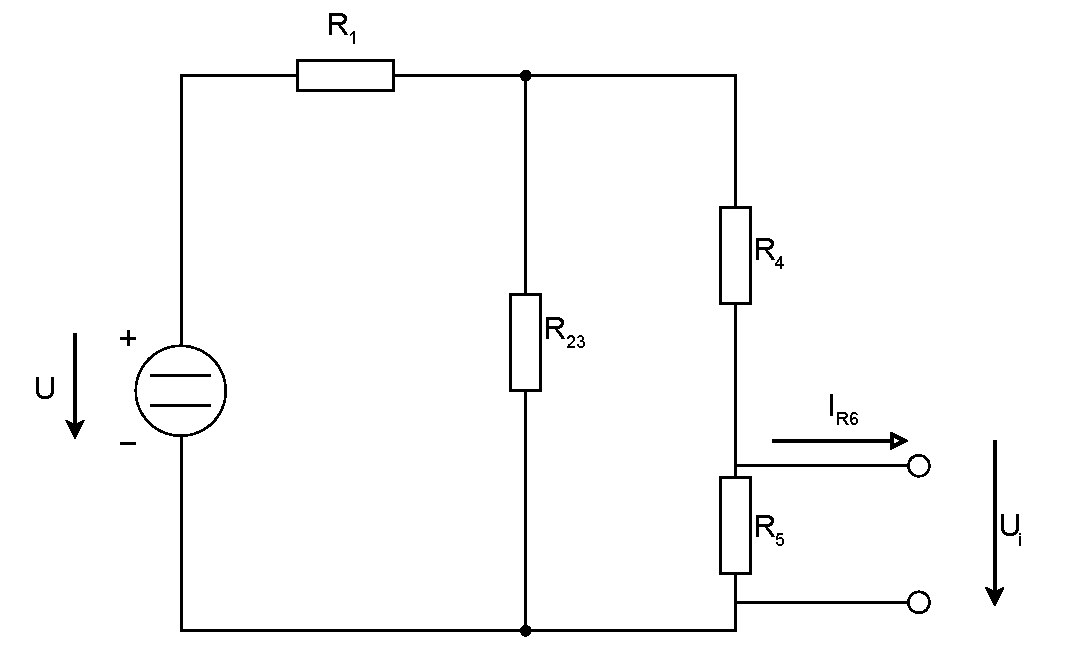
\includegraphics[scale=0.5,keepaspectratio]{fig/Pr2_1.pdf}
\[
  R_{EKV} = R_1 + \displaystyle\frac{R_{23}R_{45}}{R_{23}+R_{45}}
  = 250 + \displaystyle\frac{930 \cdot 640}{930 + 640}
  = 629.1082802547771 \Omega
\]
\[
  I = \displaystyle\frac{U}{R_{EKV}}
  = \displaystyle\frac{180}{629.1082802547771}
  = 0.28611926698390194A
\]
\[
  U_{R45} = U - (I R_1)
  = 180 - (0.28611926698390194\cdot 250)
  = 108.47018325402452 V
\]
\[
  I_{R45} = \displaystyle\frac{U_{R45}}{R_{45}}
  = \displaystyle\frac{108.47018325402452}{640}
  = 0.1694846613344133 A
\]
\[
  U_i = I_{R45} R_5
  = 0.1694846613344133 \cdot 460
  = 77.96294421383013 V
\]
\[
  R_i = \displaystyle\frac{(\displaystyle\frac{R_{23}R_{1}}{R_{23}R_1}+R_4)R_5}{
    \displaystyle\frac{R_1 R_{23}}{R_1 + R_{23}}+R_{45}
  }
  = \displaystyle\frac{(\displaystyle\frac{930\cdot 250}{930+250}+180)\cdot 460}{
    \displaystyle\frac{250 \cdot 930}{250 + 930}+640
  }
  = 207.20259188012557 \Omega
\]
Ekvivalentní obvod dle Théveninovy věty\\
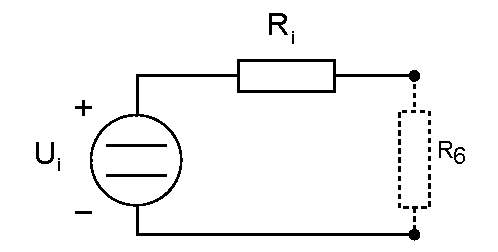
\includegraphics[scale=1.0,keepaspectratio]{fig/Pr2_2.pdf}
\[
  I_{R6} = \displaystyle\frac{U_i}{R_i + R_6}
  = \displaystyle\frac{77.96294421383013}{207.20259188012557 + 120}
  = \textbf{0.23827116944841545}A
\]
\[
  U_{R6} = R_6 I_{R6}
  = 120 \cdot 0.23827116944841545 
  = \textbf{28.592540333809854}V
\]

